\section{Audio Impedance Measurement}
%
Audio Vector Network Analysis (AVNA) measurements break into two main types,  reflection and transmission.  This section covers the first case, reflection.  The major use of reflection measurements is to determine the impedance
which creates the reflection, or, put another way, a quantity directly associated with impedance, such as inductance. This section covers AVNA impedance measurements. The next section covers transmission measurements.

The term "Vector" refers to the fact that we always measure both the amplitude and the relative phase of impedance.  This enables us to measure a combination of resistive and reactive components.
%
\subsection{Description}
Before getting to the details of the measuremets, we need to explore a few background items.

\textbf{Complex Impedance - }Using the AVNA impedance terminals, the basic measurement quantity that is often displayed is impedance described by a resistance in series with a reactance. The reactance can be either a lossless inductance or a capacitance. Mathematically, this is represented as a complex number \vecr{Z}=R+jX where R is the series resistance and X is the series reactance, both in Ohms. The AVNA uses complex-arithmetic notation for \vecr{Z} which allows mathematically sound computatiion to be done on circuit models; the user can think of it as a way to keep the resistance separate from the reactance.

If the reactance is positive, the series component represents an inductor. Likewise, if the reactance is negative, the series component is a capacitor.  Note that this is only one of many representations. As an example, a series configuration can be converted to a parallel pair of components, neither being the same value as the series pair.  We will not attempt to cover all the possibilities here, but a few of them will be described below, as they appear in the display.

\textbf{Reference Resistance - }Two differrent reference resistances can be used with the AVNA, 50 and 5,000 Ohms. The best value to use is generally the one that is in the range of the measured values. It is easy to pick 50 Ohms if the measured value is, say, 10 + j100. If the series reactance is much larger than the series resistance, we have a high-Q component that is not the easiest to measure with an AVNA. For that case we are probably going to uses the reference resistance that is closest to \(X\) since that determines the component value. If the user is trying to measure a resistance value, it is best to pick a reference resistance closest to the resistor value,

A more elaborate procedure for finding the best reference resistance for a general impedance type is to first measure with 50 Ohms. Then find the geometric mean of the resistance and the reactance, that is \(\sqrt{R X}\). Then remeasure with 5,000 Ohm reference. Choose the ratio of the geometric mean to the reference resistance (50 or 5,000) which is closest to 1.0.

Closest in all these decisions means by ratio, not by subtraction. For instance 4,000 Ohms has a ratio with 50 Ohms of  \( \frac{4000}{50} = 80\) whereas the ratio with 5,000 Ohms is \( \frac{5000}{4000} = 1.25\). The latter is closer to 1.0 than the former.  Note that we put the larger value on top of the ratio for convenience in comparing the two results.
%
\subsection{Instructions}
\textbf{Getting Started - }Here is a step-by-step description of a single frequency impedance measurement followed by a description of a swept impedance measurement. This will all be done directly from the touch screen. Everything covered here, and more, can be done via the USB-Serial link, as is described in the "AVNA Serial Control" section.

When the AVNA is powered up you have a choice of four Audio Test Instruments along with Service and Calibration functions.
\begin{figure}[H]
\begin{center}
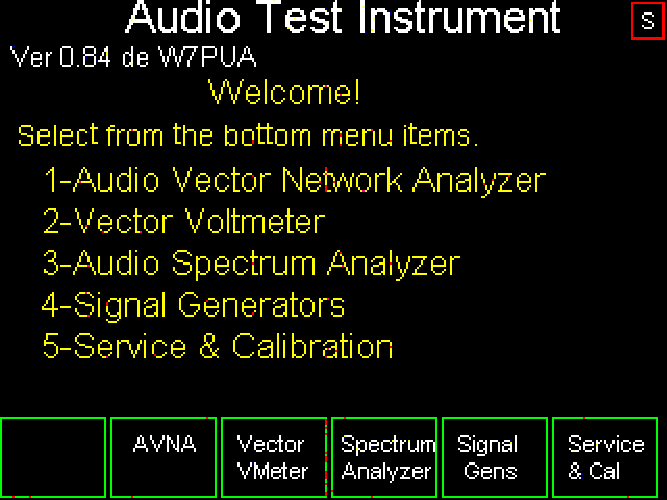
\includegraphics[scale=0.75]{./images/AVNA_000.pdf}
\caption{Audio Test Instrument Home  Screen.}
\label{AVNA_000-label}
\end{center}
\end{figure}
%
Referring to Figure \ref{AVNA_000-label}, we are now at the main Audio Test Instrument home screen. (We used to call this just, "the AVNA," but now we have added the other instruments like the Spectrum Analyzer, so this needs more descriptors.) For our impedance measurements, we will select the menu item, "AVNA" by touching that box at the bottom of the screen leading to the AVNA main screen.
\begin{figure}[H]
\begin{center}
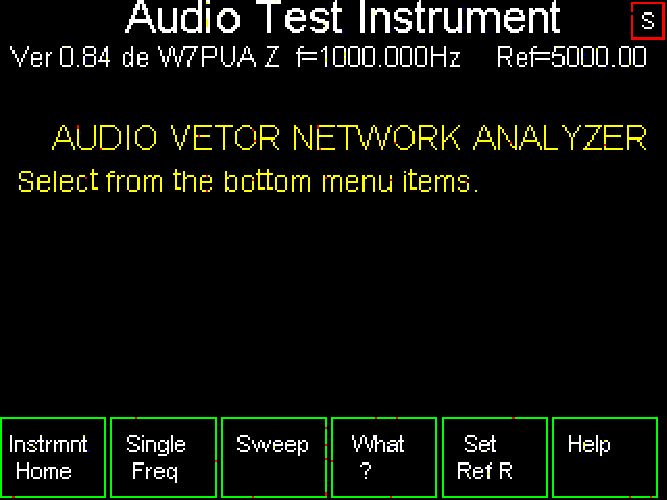
\includegraphics[scale=0.75]{./images/AVNA_001.pdf}
\caption{AVNA Main  Screen.}
\label{AVNA_001-label}
\end{center}
\end{figure}
%
We now have the choice  of single frequency or swept measurements as well a changing of the Reference Resistance described above. A last choice is the "What?" function for exploring components without knowing much about them. To continue our impedance measurement, we select "Set Ref R."
\begin{figure}[H]
\begin{center}
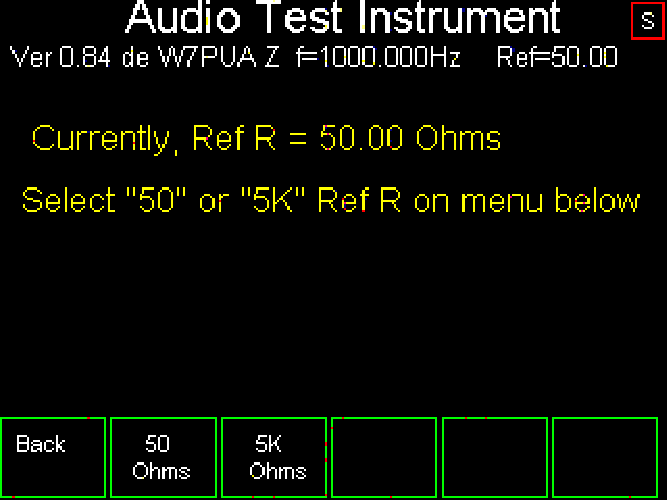
\includegraphics[scale=0.75]{./images/AVNA_003.pdf}
\caption{AVNA reference resistor selection  Screen.}
\label{AVNA_003-label}
\end{center}
\end{figure}
%
The current reference, as described above, is shown on the screen. It is also shown, during AVNA measurements, at the top of the scrren in small type. Selecting the current value has no effect, and so we choose the menu item, "5k Ohms."
\begin{figure}[H]
\begin{center}
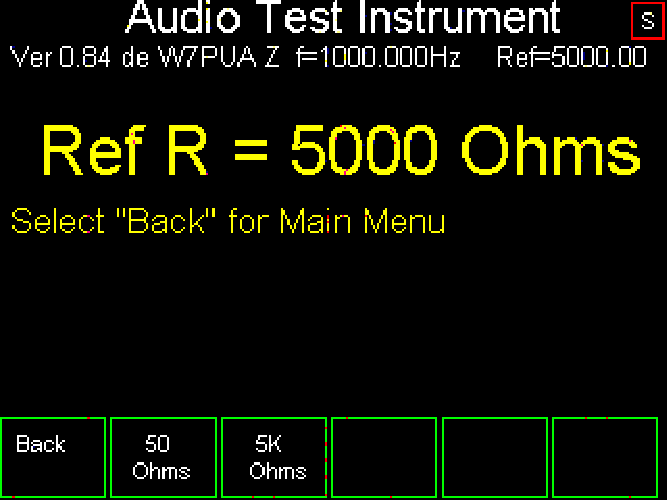
\includegraphics[scale=0.75]{./images/AVNA_004.pdf}
\caption{AVNA reference resistor selection of 5000 (5K) Ohms.}
\label{AVNA_004-label}
\end{center}
\end{figure}
At this point we have chnged the reference resistance and can return to the AVNA main screen, Figure \ref{AVNA_001-label}, by tapping the menu item, "Back."

\textbf{Measuring an Impedance - }As an example: put together a series combination of a 10 Ohm resistor and a 0.22 $\mu$F capacitor and put this across the Z terminals. To get started, we can measure this at a single frequency by tapping on the menu item, "Single Freq." The frequency can be selected from a list of 13 ranging from 10 Hz to 40 kHz by using the menu items, "Freq Down" and, "Freq Up."  For this sample measurement set the frequency to "1000 Hz".  Next, the menu item, "Meas Z" is tapped to start a continuing series of impedance measurement, as shown next.
\begin{figure}[H]
\begin{center}
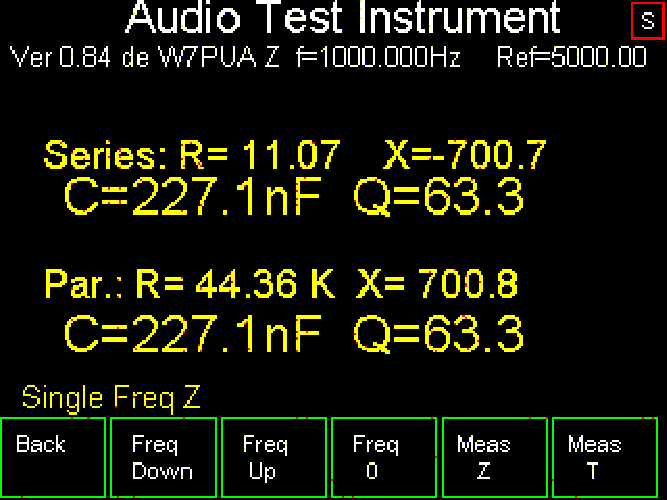
\includegraphics[scale=0.75]{./images/AVNA_006.pdf}
\caption{Impedance measurement of a series combination of 10 Ohms and a 0.22 $\mu$F capacitor.}
\label{AVNA_006-label}
\end{center}
\end{figure}
A couple of items to note.  First, this measurement repeats every second or so.
This is useful if you are measuring multiple components, or if you want to do mental averaging of the component values.

Next, we see the series combination of  \vecr{Z}=11.07 -j700.7, which is the resistance and reactance. I measured the 10 Ohm resistor, without the capacitor and saw 9.81 Ohms with a 50 Ohm reference an 8.23 Ohms with a 5000 Ohm reference, so the 11.07 value which is probably a combination of the difficulty in measuring the resistor with 700 Ohms reactance in series as well as some loss in the capacitor.  The 9.81 Ohms is very close to the measured DC value. Then we see the translation of the reactance value to a capacity of 227.1 nF (or 0.2271 $\mu$F).  Often this is the value we are looking for.

The Q value shown of 63.3 is the ratio of the reactance magnitude to the resistance value.  We are accustomed to measuring Q of inductors, and that would be shown here if the reactance was positive.  The Q of a capacitor has the same physical meanings as inductors.

Lastly, the same screen shows the parallel RC values. At the one frequency where we measure the series connected components, we could have connected this parallel combination, and we would have measured the same quantities.
For more details on the series/parallel equivalence, see the original QEX article.\footnote{http://www.janbob.com/electron/AVNA1/Larkin-QEX-2018-May-Jun.pdf pg. 12}
%
In particular, note that, in general, both the resistance and reactance values will change between the series and parallel representations.

\textbf{Swept Impedance Measurements - }  We do not have a graphical presentation of frequency swept impedance data.  Instead we have a tabular listing. To do this measurement from the single frequency version, we tap on "Back," bringing back the screen of Figure \ref{AVNA_001-label}. At this point we could change the reference resistor to 50 Ohms, but will not for this exercise. Instead, we tap on "Sweep," bringing up the following screen.
\begin{figure}[H]
\begin{center}
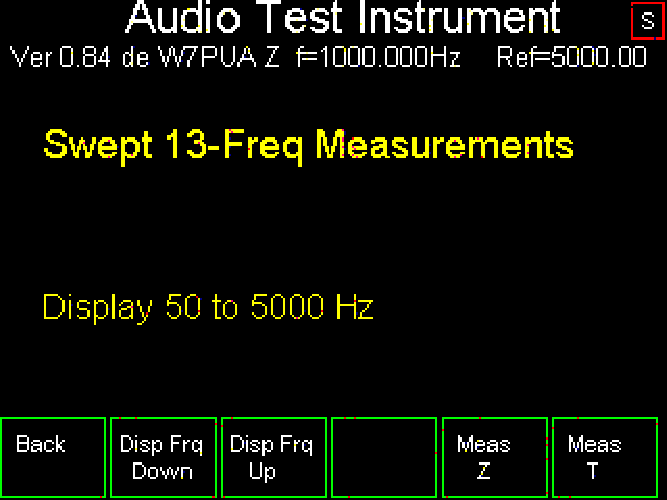
\includegraphics[scale=0.75]{./images/AVNA_007.pdf}
\caption{Mainscreen for swept measurements.}
\label{AVNA_007-label}
\end{center}
\end{figure}
We can change the 7 screen displayed frequencies with the two menu items at the bottom.  In all cases, the measurements are made at all 13 frequencies, but there is not room to display them all.  For now, we will leave the frequency settings at 50 to 5000 Hz.  We command the impedance measurement by tapping on, "Meas Z."  Here is the display.
\begin{figure}[H]
\begin{center}
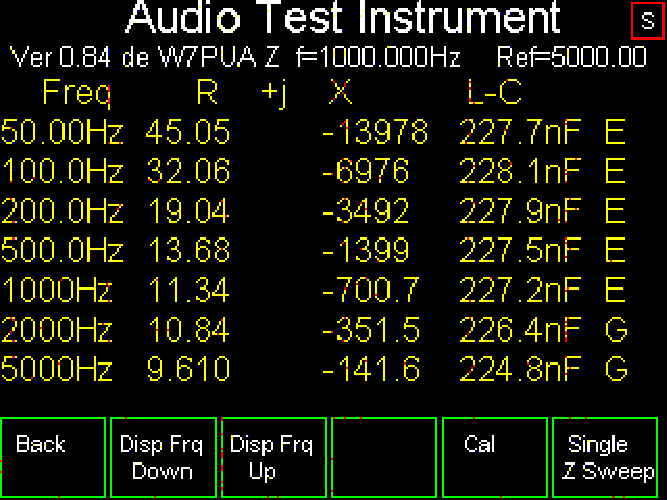
\includegraphics[scale=0.75]{./images/AVNA_009.pdf}
\caption{Swept impedance measurements.}
\label{AVNA_009-label}
\end{center}
\end{figure}
%
The display shows the impedance for seven frequencies.
The menu items, "DispFrq Down" and "DispFrq Up" allow the displayed frequencies to be shifted down or up to cover the entire 10 to 40,000 Hz range.  The impedance is shown in  \(R+jX\) format. It can be seen that negative reactance values display with a minus sign in front of the value. Next in the display line is a translation of the  \(jX\) value to either a capacitance or inductor value. The units, in this case,  "nF" change with component value.  In the right hand column is a rough measure of measurement quality. A single letter E, G, P corresponds to (E)xcellent, (G)ood, or (P)oor. These indicate the difference between the impedance and the reference resistance.
They should not be taken too literally, but if the letter shows "P" or even "G",  you might consider the values and whether to re-measure with the other reference resistance.

Going back to the AVNA main menu, there is a menu item, "What?".  This is handy if the component type or value is unknown, or maybe a quick answer is wanted.  This starts with the following menu that describes what to do.
\begin{figure}[H]
\begin{center}
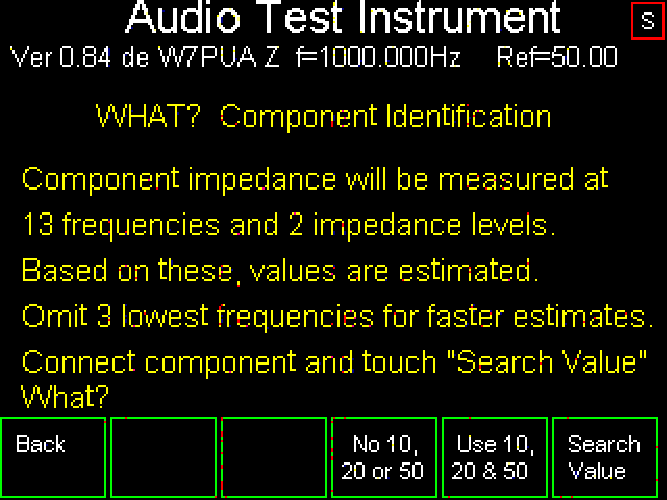
\includegraphics[scale=0.75]{./images/AVNA_012.pdf}
\caption{AVNA What? Screen.}
\label{AVNA_012-label}
\end{center}
\end{figure}
%
The only option available is to omit measuring at 10, 20 and 50 Hz that speeds up the measurement.
Otherwise, tapping on "Search Value" produces the estimate:
\begin{figure}[H]
\begin{center}
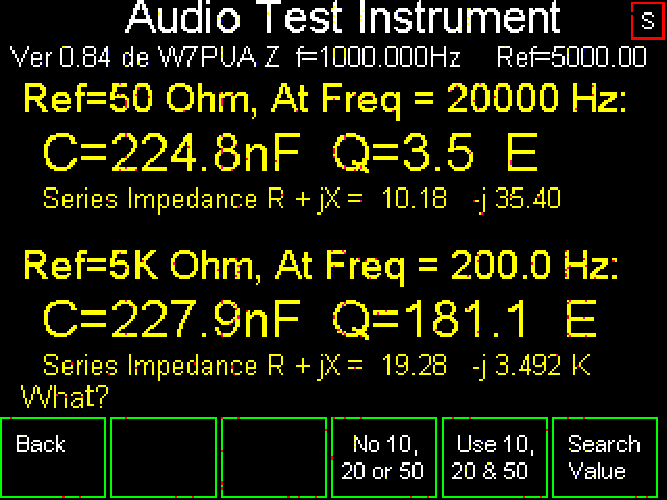
\includegraphics[scale=0.75]{./images/AVNA_013.pdf}
\caption{AVNA What? Screen after measuring.}
\label{AVNA_013-label}
\end{center}
\end{figure}
%
Two different values are shown, corresponding to the two reference resistor values.  The "What?" process chooses the frequency that gives an "E" for excellent measuremnt, if possible.  Often, this differs in frequency between the two reference resistor values.  For our 10 Ohm and 0.22 $\mu$F series combination, we find the 50 Ohm reference measurmeny at 20,000 Hz and the 5000 Ohm measurement down at 200 Hz.  In either case, the capacity value works out well, but measuring the 10 Ohm resistor in series with a 3492 Ohm reactance (at 200 Hz) is looking less successful with a 19.28 indicated \(R\) value.  It would be interesting to explore this further by measuring the two components individually with swept measurements.  But we won't do that here to save the fun for others.
%
\subsection{Discussion}
%
\textbf{Measurement Technique - } There are two commonly used methods of measuring impedance, the unbalanced Wheatstone bridge
%
\footnote{The classic Wheatstone bridge, https://en.wikipedia.org/wiki/Wheatstone\_bridge}
\footnote{The Wheatstone bridge in various AC/RF forms,\\ \hspace*{1.0 in}{http://g3ynh.info/zdocs/bridges/part\_1.html}}
%
 and the series resistor method.   The latter method is used in the AVNA.
\begin{figure}[H]
\begin{center}
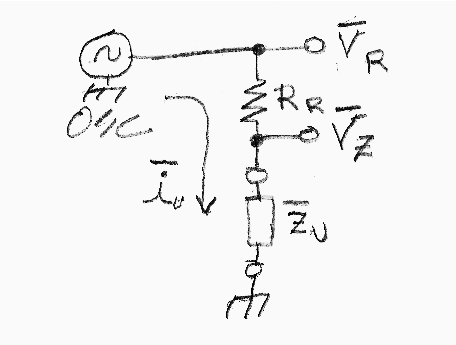
\includegraphics[scale=0.75]{./images/AVNA_900.pdf}
\caption{Functional schematic of impedance measuring circuit.}
\label{AVNA_900-label}
\end{center}
\end{figure}
Figure \ref{AVNA_900-label} shows the deceptively simple measurement circuit.  A software Direct Digital Synthesis (DDS) in the Teensy DSP creates a sine wave signal at a frequency between 10 and 40,000 Hz.  This is converted to an analog voltage by the left DAC on the Teensy Audio Adapter board which then goes to an audio amplifier producing the analog signal  \vecr{$v_R$} seen on the diagram.
The overhead bar indicates that this is a complex voltage where we care about the phase of the sine wave as well as the amplitude.  \vecr{$v_R$} is applied to the series combination of our reference resistor, \(R_R\) and the unknown impedance, \(\bar{Z_u}\).  This results in a current through the pair  of \(\bar{v_R}/(R_R + \bar{Z_u})\).  By measuring the complex voltage at the top of the unknown, \(\bar{v_Z}\) we can determine this current as
\begin{equation}
 \bar{i_u}=(\bar{v_R} -\bar{v_Z})/R_R
\end{equation}
 This in turn allows calculating the unknown impedance as
\begin{equation}
 \bar{Z_u} = \bar{v_Z}/\bar{i_u}
                    = \bar{v_Z}/(\bar{v_R}-\bar{v_Z})/R_R
\end{equation}
As one would expect, this requires knowledge of the reference resistor value, but the absolute voltages are not used, but rather the ratio of absolute voltages.  This makes it important to have the two voltmeters, \(\bar{v_R}\) and \(\bar{v_Z}\) track in both amplitude and phase.  There is separate analog circuitry in the two voltmeter paths, so errors will occur.  These errors are removed by the calibration procedure where the two voltmeters are connected to the signal source and the ratio  of voltages and the difference in phase of the two is recorded. These are then applied as corrections at each impedance measurement.

\textbf{Measuring Amplitude and Phase - }The discussion of Measuring Technique, above, refers to the two voltmeters that are needed.  Most of the  implementation of voltmeters is discussed in the QEX article.\footnote{http://www.janbob.com/electron/AVNA1/Larkin-QEX-2018-May-Jun.pdf pg 8-9}
%
and won't be repeated here.  The basic process is to generate a pair of software sine waves that are 90 degrees apart in phase but at the exact measurement frequency.  Each of these is multiplied (mixed) with the signal being measured and then low-pass filtered.  This produces the two complex voltages, needed for the impedance calculation.  All of the mixing and filtering occurs in the Teensy DSP.